%&tex
\chapter{Introduction}\label{sec:introduction}
	Computer vision is the scientific endeavour to algorithmically understand patterns in images.
	Structures and processes in the physical world interact in complex ways to generate an image. The image then acts as a mirror, in which these elements of the world are reflected and leave patterns.
	To recognize patterns in an image, means in essence to observe the reality lurking behind this mirror, \ie to measure the causal elements that contributed to the image generation.


	In this thesis, we focus on our efforts on image datasets which feature a single object class.
	Typically, objects appear in an intricated interaction of many factors of variation.
	For example, in an image dataset of people, the persons can vary in their visual appearance by clothing and skin color or in their geometric structure due to their pose or body physique.
	% The image generation process itself may further add factors like illumination, viewpoint or contrast.
	The two prominent factors of variation for articulated objects are geometric shape and visual appearance.
	Disentangling these factors is a difficult problem, due to the intricated interplay of shape and appearance, especially under heavy articulation.
	The complexity enters, as a variation in shape is a change of the images domain rather than a change of its values~\cite{shu18shapeappear, xing18shapeappear}.
	Consider a person raising his arm: the color and texture of his pullover sleeve intrinsically does not change, but appears at a different location in the image. An efficient model for shape should cover all possible states of the object and preserve the local linkage to its intrinsic appearance.

\section{Why Disentangle Causal Factors?}
	Above, we framed disentangling generative factors as similar to a scientific measurement process. An interaction of physical elements in the world is captured in an image, which can be treated as a scientific measurement of reality. Discerning patterns, and disentangling sources of patterns from each other, will then be defined as \textit{understanding} the world. What can be gained from such an \textit{understanding}?
	On the one hand, there are pragmatic reasons to aim at extracting disentangled factors from images: to successfully transfer a representation between different tasks, typically only a few factors are relevant \cite{bengio13rep}.
	Efficient transfer and multi-task learning should account for this.
	On the other hand, learning to capture external mechanisms in appropriate internal representations, can be seen as a step to automate visual reasoning itself.
	Once disentangled, a factor can be manipulated individually to make a targeted change in an image. Thereby, not only humans may change images at will, but also machines may reason about the world \cite{pearl18impediments}, by simulating changes to factors internally in their model of the world.
	Thought experiments like \textit{"imagine, how ridiculous you would look, if you wore that hot pants"}\note{creepy} are manageable tasks for the human imagination, but are out of the league for currently used generative image models \cite{goodfellow14gan, kingma13vae}, that typically rely on non-interpretable vector spaces with entangled dimensions.
	Building imagination machines has been proposed as a goal for artificial intelligence research recently \cite{mahadevan18imagine}.
	% To imagine, is to manipulate of an internal model to generate internal images.
	In this sense, in the context of generative modelling, disentangling factors could as well lead the way from a science of images to a science of imagination.
	% \note{Data-driven algorithms for pattern recognition good recently}
	% \note{how much and how to incorporate prior knowledge}
	% \note{is this necessary, theoretical arguments against}
	% \begin{itemize}
		% \item Computer vision: automatically discern patterns, that reflect structures in physical world
		% \item Why disentangle: detect causal factors to image
		% \item Pragmatic reason: efficient transfer learning, multi-task learning
		% \item Philosophical reason: build machines that understand mechanisms, reason about world \cite{Pearl:2018im}
		% \item Targeted changes $\rightarrow$ thought experiments; not possible for e.g. GAN, VAE\ \textit{"imagine, ..."}\ science of images $\Rightarrow$ science of imagination \cite{Mahadevan:2018tz}.
	% \end{itemize}

\section{How not to Disentangle.}
	\begin{figure}[t]
		\centering
		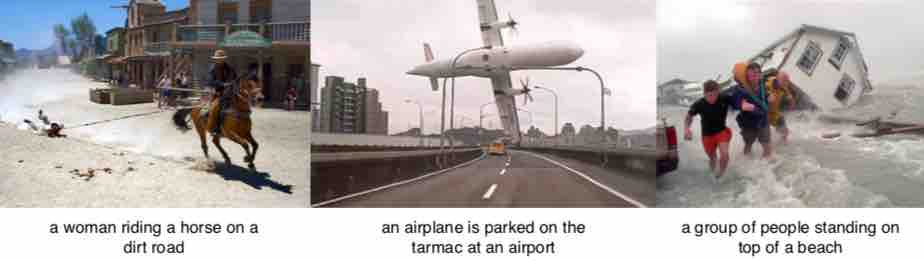
\includegraphics[trim={0cm 0cm 0cm 0cm},clip, width=1.\linewidth]{fig/other/notcausal}
		\caption{The image captions are generated by a deep neural network (Neuraltalk2) \cite{karpathy15neuraltalk}. Yet, common sense understanding of psychological and physical entities in terms of causal relationships and narratives is absent \cite{tenenbaum18think}. Instead, the neural network seems to capture mere associations.}
		\label{fig:notcausal}
	\end{figure}
	Can machines tell a story? Carefully observe your own mind, when viewing the images shown in Fig. \ref{fig:notcausal}: observe how the human mind immediately interprets and jumps to conclusions, tries to tell itself a story that explains an image, whereas the machine (in this case, NeuralTalk2 \cite{karpathy15neuraltalk}), is comically descriptive in contrast.
	The missing \textit{common sense} may be due to a missing causal reasoning, due to a missing disentangled causal representation of the world.
	But how to learn a disentangled representation from scratch, \ie from raw image data?
	As we will find out (in Sec. ~\ref{sec:causality}), disentangling causal factors from raw image data, without any side information is impossible theoretically.
	% , and can only work based on interaction assumptions.

	Lets consider an example: Given an image dataset of human persons, that has strong variation in the pose and in the appearance of the persons, how to find these two underlying axes of variation (pose and appearance)? Lets suppose the distribution of variation follows a two-dimensional Gaussian distribution, one dimension for pose, one for appearance.
	The learning algorithm has access to randomly sampled images from this distribution. An intelligent data compression algorithm will be able to fit a function from the images to the two-dimensional subspace, which explains (by assumption in this example) the variation in the dataset.\todo{plot two-dimensional Gaussians}
	But are the two dimensions, that the algorithms finds disentangled? No. In fact, any linear combination of pose and appearance axes and its orthogonal complement are equally valid to span the subspace of underlying variation. Just from observing a two-dimensional Gaussian, no meaning will be attached to the axes. In practice, this problem is often circumvented by first fitting a generative model to the image dataset and \textit{afterwards} interpolating in the latent space to determine (by human judgement) the axes of interest (here the pose or appearance axis). The meaning of pose and appearance as independent factors comes from the fact, that it is easily possible in the real world to change one factor without the other. A person moving without loosing clothes is a trivial example for that.
	In summary, on the basis of dataset statistics alone one cannot disentangle causal factors, if the information about how to select the axes, \ie which factors to separate, is not contained in the raw data.
	Fitting a model to the data distribution, does in general not give insight into how the data was generated.

\section{How can Humans Disentangle?}
% \section{What can Machine Learning Learn from Humans?}
	The dichotomy between humans and machines is constructed, of course, because on a fundamental level humans are machines.
	\note{explain and state performance gap in lacking reasoning, causal discovery, }
	But in this context, the distinction between humans and machines shall refer to the current gap between human and machine learning performance, in terms of inferring generative factors and reasoning (again, cf. Fig. \ref{fig:notcausal}).
	So, what advantageous characteristics does the human mind have, that are lacking in data-driven machine learning algorithms?

	\emph{Priors.}
		Whether acquired or inherited, certain inductive priors seem to guide the human learning in its early phases \cite{tenenbaum18think}.
		Archetypal knowledge of psychology \cite{jung68archetype}, a universal grammar for language \cite{chomsky00horizons} and causal intuitions on everyday physics \cite{teglas11intuitive} are some of the cognitive priors, that could explain the intuitive psychology, the rapid language acquisition and the remarkable causal inference from limited amount of data.

	\emph{Data.}
		Not only quantity, but also quality of data. Machine learning on images is commonly posed as the task to learn from randomly sampled images from a data set. But humans do not perceive the world in arbitrary samples.
		To humans, the world appears in a temporal sequence, which reveals how generative factors change and persevere across time. Instead of focusing on datasets with static images, sampled at random so that the images may have nothing to do with each other, algorithms should use video datasets and harness the rich temporal information.\\
		Another key difference is, that humans interact with their environment.
		That means, humans know change, not only by observing change (as in a temporal sequence), but also by changing.
		Anyone, who has watched a human infant play, can affirm that the learning mind is obsessed with interaction and change. The inevitable destruction around a young human is no accident, but a result of curious learning.
		\note{Whether consciously by performing controlled experiments or by subconscious cues \cite{wall08egomotion}:}
		\textit{Interaction is crucial for a learning mind.}

		% causal inference
		% 3. Learning by interacting: knowing change by changing.
		% second rung on causal ladder (Pearl): intervention. (, acting) What happens if I do?
		% P(s, do(a))
		% Others: counterfactual (imagining), association.
		% In humans e.g. egomotion cues: how does image on retina change if I move.

	\emph{Models.}
	% humans what model: imagination: e.g.
		Humans are able to imagine. That presupposes an internal model of the world, to which specific changes of representational factors can be applied.
		% So-called dreaming neural networks can distract from the fact that human imagination is make changes to the world that it did not observe.
		In machine learning, fitting neural network models as functions to approximate datasets has seen tremendous progress recently, to the point, that it is considered a solved problem \todo{cite something, maybe bigGAN etc)}. This progress is mainly due to the effectiveness of neural networks to fit high-dimensional functions. But a probabilistic fit to a dataset, however complex and rich, is not a causal model. Even if one were to obtain a probabilistic model over all images the world (one could start with \eg ImageNet \cite{russakovsky15imagenet}), this would tell very little about the real-world (causal) relationships between objects.
		\note{One could hope for relationships to emerge by data compression alone, but }
		\note{A step towards intelligence would be to automate the finding of "meaning" in the learned latent spaces. But meaning has to come from somewhere, and will not emerge from the data itself.}

	What can we learn from these differences? An algorithm to understand the world: should contain useful \textit{prior} assumptions to efficiently use \textit{data} that contains the necessary causal relationships and interactions, to learn a useful \textit{model} of the world.

% \section{How to Disentangle?}
	% change factor $\rightarrow$  image change equivariantly, leave others invariant
	% $\rightarrow$  equivariance, invariance
%
	% change can be mimicked artificially
	% Intelligent pattern recognition algorithms, fuelled by sensory data as learning material alone, may ultimately drive the way to a full-blown artificial intelligence, reasoning about the world on its own. - That is the reasoning behind data-driven and assumptionless machine learning approaches that have conquered several research communities.
	% A theoretical objection to driving-only-with-data comes from the causal literature: For an understanding of the world, an algorithm needs to model causal processes, that cause an image to be generated.

\section{Contributions}
	This thesis makes two theses:
	\begin{itemize}
		\item  \textit{Hypothesis \emph{i)}: Unsupervised learning of object shape benefits from abstracting away the complement of shape, namely the object appearance. Explaining away the appearance factor can be achieved by a disentangled generative modelling of both factors.}
		\item \textit{Hypothesis \emph{ii)}: Learning unsupervised disentanglement without any assumptions is fundamentally impossible. In accordance with the literature on causal learning \cite{pearl18impediments}, disentangling causal factors requires model assumptions and/or interactional data - instead of observational (raw) data.}
	\end{itemize}
	% \emph{ii)} Following the need to interact with the world, need to change, need to model physical reality -> image transformations, analyis-by-synthesis}
	To address these hypotheses, we \textit{explain}, \textit{validate} and \textit{evaluate} a method for unsupervised shape learning: \textit{Unsupervised Part-wise Disentanglement of Shape and Appearance} developed by Lorenz \etal\ 2018\todo{cite properly}.


	To \textit{explain}, we give an overview over state-of-the-art unsupervised disentangling literature and situate the proposed method in relation to the literature. In particular, we carve out the necessary aspects of an approach for disentangling causal factors and analyze the current state of research in order to indicate future directions.


	To \textit{validate}, we show that the proposed method outperforms the state-of-the-art for unsupervised learning of object shape on miscellaneous datasets, featuring human and animal faces and bodies.
	We also contribute several self-made video datasets for disentangling human pose from appearance, for articulated animal motion and for articulated composite objects. We highlight the specific challenges of these datasets and elucidate how the proposed method tackles them.


	To \textit{evaluate}, we perform ablation studies on critical components of the method. In addition, we compare to a part-wise shape learning method which does make the goal of disentangling explicit.
	To show that the disentanglement is indeed achieved, we evaluate the disentanglement performance against a shape-supervised state-of-the-art disentanglement method and perform favorably.


	In short, our results are a big improvement upon the state-of-the-art in unsupervised object shape learning. This confirms the first hypothesis. To complement the learned shape in a generative process, object appearance is disentangled from shape. The achieved disentanglement with our causal assumptions, and the not-achieved disentanglement when dropping these assumptions, confirms the second hypothesis.
